\documentclass{standalone}
\usepackage{tikz}
\usetikzlibrary{shapes.geometric, arrows.meta}

\tikzset{
    block/.style = {rectangle, draw, text width=6em, text centered, minimum height=3em},
    line/.style = {draw, -Stealth}
}

\begin{document}

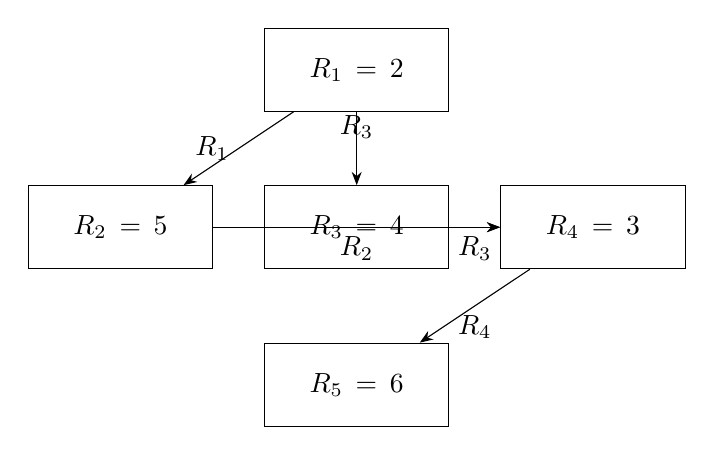
\begin{tikzpicture}[node distance=2cm]

\node (R1) [block] at (0, 0) {$R_1 = 2$};
\node (R2) [block] at (-3, -2) {$R_2 = 5$};
\node (R3) [block] at (0, -2) {$R_3 = 4$};
\node (R4) [block] at (3, -2) {$R_4 = 3$};
\node (R5) [block] at (0, -4) {$R_5 = 6$};

\draw [line] (R1) -- node[anchor=east] {$R_1$} (R2);
\draw [line] (R1) -- node[anchor=south] {$R_3$} (R3);
\draw [line] (R2) -- node[anchor=north] {$R_2$} (R4);
\draw [line] (R3) -- node[anchor=north] {$R_3$} (R4);
\draw [line] (R4) -- node[anchor=north] {$R_4$} (R5);

\end{tikzpicture}

\end{document}